\section{Background}
\label{cha:lit-review}

\subsection{Steganography and Steganalysis}
\label{sec:lit-review:stego}

Confidentiality has been well established as a security
criterion \cite{gollmann}.  Essentially, confidentiality is the preservation of
authorized access and disclosure to information \cite{fips-199}.  In most
cases, confidentiality is sufficient for protecting information from disclosure.
For example, when using online banking, it is important to conceal the contents of the
communications so that no others can impersonate either yourself or the bank or
otherwise obtain your private banking information, but it is not usually
important to hide the fact that you are performing the online banking.
However, there are situations where it is not only important to hide the
contents of communication, but also the fact that communication has taken place
at all.  This is the \emph{undetectability} criterion of security, defined by
Pfitzmann and Hansen \cite{anon_terminology} as the criterion of being able to
determine if a message even exists.

Just as cryptography is the science related to confidentiality, \\steganography is
the science related to undetectability \cite{steganalysis}.  Also, as
cryptanalysis is the analysis of cryptographic techniques and how to break
them \cite{comp-sec}, steganalysis is the study of steganographic techniques
and finding hidden information \cite{steganalysis}.  From the definitions of
both cryptography and cryptanalysis, we can deduce that a cryptographic system can be
considered broken when an attacker can determine the contents of the
communication, also called the plaintext.  Therefore, we can consider a
steganographic system (stego system) broken when an attacker can determine that
secret communication has taken place, that is the attacker has \emph{detected}
the communication, even if they have not determined the contents of the
message \cite{steganalysis}.

\subsection{Botnets}
\label{sec:lit-review:botnets}

Botnet software is a type of malicious software (malware) that is most often
placed on a victim's computer silently.  Unlike traditional malware, however,
the botnet software communicates with a botmaster or bot-herder that coordinates
potentially thousands or even millions of other infected machines, called bots or zombies,
in other attacks.  Once created, a botnet can be used for harvesting personal
information on a global scale, or causing significant denial of service attacks
to even the largest organizations \cite{botnet-ecosystem}.

Every botnet must have a command and control (C\&C) system that directs the
bots to perform their attacks.  Zeidanloo and Manaf \cite{botnet-cc-mechanisms} have
separated botnet C\&C systems in to three groups.  Some botnets use centralized C\&C
centers where the botmaster can control all bots directly.  Other botnets use a
peer to peer C\&C system, where bots communicate with each other.  In addition
to receiving commands, many botnets must communicate information back to the
botmaster, especially if their goal is to obtain the private information of the
user whose computer hosts the botnet software.  Finally, some botnets use a
hybrid approach.

In the centralized model, communication between the bots and botmaster is
often done using an IRC channel or over HTTP.  This was the original botnet C\&C
model used.  Because the system is centralized, the C\&C center acts as a single
point of failure for the botnet.  When using IRC, the botmaster will create an
IRC channel on their server and the bots will then connect to the server to
communicate with the botmaster.  From this IRC channel, the botmaster could
command all bots to initiate a DDoS attack on an enemy.  If the botnet
communicates over HTTP, it gains the advantage that HTTP traffic is not
suspicious in general, because it is the protocol used for web traffic
\cite{botnet-cc-mechanisms}.  A centralized approach may also
maintain several C\&C centers to improve communications and prevent having
a single point of failure, as shown in figure
\ref{fig:lit-review:botnets:centralized-multiple}.

\begin{figure}
\centering
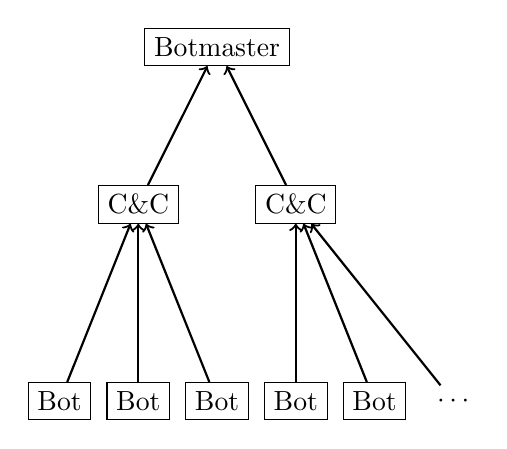
\begin{tikzpicture}
    \node[draw] (m1) {Bot};
    \node[draw] (m2) [right of=m1,node distance=1cm] {Bot};
    \node[draw] (m3) [right of=m2,node distance=1cm] {Bot};
    \node[draw] (m4) [right of=m3,node distance=1cm] {Bot};
    \node[draw] (m5) [right of=m4,node distance=1cm] {Bot};

    \node[draw] (m) [above of=m3,node distance=4.5cm] {Botmaster};
    \node[draw] (cc1) [above of=m2,node distance=2.5cm] {C\&C};
    \node[draw] (cc2) [above of=m4,node distance=2.5cm] {C\&C};

    \draw[->,thick] (m1) -- (cc1);
    \draw[->,thick] (m2) -- (cc1);
    \draw[->,thick] (m3) -- (cc1);
    \draw[->,thick] (m4) -- (cc2);
    \draw[->,thick] (m5) -- (cc2);
    \node (dots) [right of=m5,node distance=1cm] {$\cdots$};
    \draw[->,thick] (dots) -- (cc2);

    \draw[->,thick] (cc1) -- (m);
    \draw[->,thick] (cc2) -- (m);
\end{tikzpicture}
\caption{Botnet C\&C for a centralized botnet with multiple C\&C centers.}
\label{fig:lit-review:botnets:centralized-multiple}
\end{figure}

Although most botnets use IRC or HTTP to communicate directly, the botnet
designed for this paper will communicate over a social network.  This concept
has been discussed in some previous work, for example in \cite{twitter-botnet},
a method of C\&C over Twitter is discussed, however the commands are sent
directly as the content of the tweets instead of by using a covert channel.  A
botnet has been designed to use steganography over a online social network
\cite{stegobot}, but it uses image steganography to embed messages in the images
posted normally by the victim.  It requires that other bots in the botnet be on
computers socially connected to the victim via the online social network.
